\documentclass[11pt,a4paper]{article}

\usepackage[margin=1in]{geometry}
\usepackage[T1]{fontenc}
\usepackage[utf8]{inputenc}
\usepackage{amsmath,amssymb}
\usepackage{graphicx}
\usepackage{booktabs}
\usepackage{xcolor}
\usepackage{listings}
\usepackage[hidelinks]{hyperref}

% Keep fig1.png in the same folder as this .tex file.
\graphicspath{{./}}

\lstdefinestyle{cudaStyle}{
    language=C++,
    basicstyle=\ttfamily\small,
    keywordstyle=\bfseries\color{blue!60!black},
    commentstyle=\itshape\color{gray!70!black},
    stringstyle=\color{red!60!black},
    numbers=left,
    numberstyle=\tiny\color{gray},
    frame=single,
    breaklines=true,
    columns=fullflexible,
    showstringspaces=false,
    tabsize=4
}
\lstset{style=cudaStyle}

\title{CUDA Chapter 5 Notes: Sections 5.1--5.4\\
Memory Access Efficiency, CUDA Memory Types, and Tiled Matrix Multiplication}
\author{}
\date{}

\begin{document}
\maketitle

\section{The Main Task of Chapter 5}

The previous chapters focused mainly on how CUDA organizes and schedules parallel work: grids contain blocks, blocks contain threads, and threads are executed in warps on streaming multiprocessors. Chapter 5 shifts the focus from \emph{how many threads are running} to \emph{how efficiently those threads obtain and reuse data}. The central objective is simple:

\begin{center}
\fbox{\parbox{0.88\textwidth}{
\textbf{Every value fetched from global memory should support as much useful computation as possible.}
}}
\end{center}

This matters because global memory is large but relatively expensive. Arithmetic hardware can execute operations very quickly, but it cannot do useful work until the required operands have arrived. Chapter 5 therefore connects memory behavior, computational intensity, the Roofline model, the CUDA memory hierarchy, and finally shared-memory tiling.

\section{Latency, Bandwidth, and Why Memory Can Limit Performance}

\textbf{Memory latency} is the delay between issuing a memory request and receiving the requested value. A global-memory access may require many clock cycles. GPUs tolerate this delay through \textbf{latency hiding}: when one warp is waiting for data, the SM scheduler can issue instructions from another ready warp whose state is already resident on the SM. In this way, a long latency does not necessarily mean that the entire SM must remain idle.

\textbf{Memory bandwidth}, in contrast, is the maximum amount of data that can be transferred per unit time. If a device can deliver at most $B_{\max}$ bytes per second, launching additional warps cannot raise the sustained transfer rate beyond that physical limit. More resident warps can hide latency, but they cannot eliminate a bandwidth bottleneck. Once the memory system is saturated, the only fundamental way to obtain substantially more arithmetic throughput is to \textbf{perform more useful work per byte transferred}.

\section{Naive Matrix Multiplication and Computational Intensity}

Consider

\[
    P = MN,
\]

where $M$, $N$, and $P$ are square matrices. One CUDA thread computes one output element

\[
    P_{row,col}
    =
    \sum_{k=0}^{\texttt{Width}-1}
    M_{row,k}N_{k,col}.
\]

For a fixed thread, $row$ and $col$ remain unchanged while $k$ moves through the shared dimension. Therefore, that thread reads \textbf{one row of $M$ and one column of $N$} and forms their dot product.

In each iteration of the dot product, the thread reads one single-precision value from $M$ and one from $N$. Since one \texttt{float} occupies $4$ bytes, the iteration transfers

\[
    2\times 4 = 8\ \text{bytes}
\]

from global memory. The same iteration performs one multiplication and one addition, which are counted as

\[
    2\ \text{FLOPs}.
\]

The accumulator is normally kept in a register, so it does not require a global-memory access in every iteration. The final output is also written only once after the complete dot product. The dominant repeated traffic is therefore the two input loads.

The \textbf{compute-to-global-memory-access ratio}, also called computational or arithmetic intensity, is

\[
\boxed{
    I
    =
    \frac{\text{useful floating-point operations}}
         {\text{bytes transferred from global memory}}
}
\]

and is measured in FLOP/B. For the naive matrix-multiplication inner loop,

\[
    I_{\text{naive}}
    =
    \frac{2\ \text{FLOPs}}{8\ \text{B}}
    =
    0.25\ \text{FLOP/B}.
\]

This is a very low intensity: a large amount of data movement supports only a small amount of arithmetic.

\subsection{A100 example}

Using the textbook A100 example with peak memory bandwidth

\[
    B_{\max}=1555\ \text{GB/s},
\]

the bandwidth can support at most approximately

\[
\begin{aligned}
    P_{\text{memory}}
    &= B_{\max}I_{\text{naive}} \\
    &= 1555\times 0.25 \\
    &\approx 389\ \text{GFLOP/s}.
\end{aligned}
\]

This is far below the stated ordinary FP32 peak of about $19.5$ TFLOP/s. The important conclusion is not the exact percentage, but the architectural principle:

\begin{center}
\fbox{\parbox{0.88\textwidth}{
\textbf{Powerful arithmetic hardware is useful only when the memory system can supply enough data, or when each fetched value is reused enough times.}
}}
\end{center}

\section{The Roofline Model}

The Roofline model combines the two major upper bounds on kernel performance: the maximum rate at which memory can deliver operands and the maximum rate at which the GPU can execute arithmetic.

\begin{figure}[htbp]
    \centering
    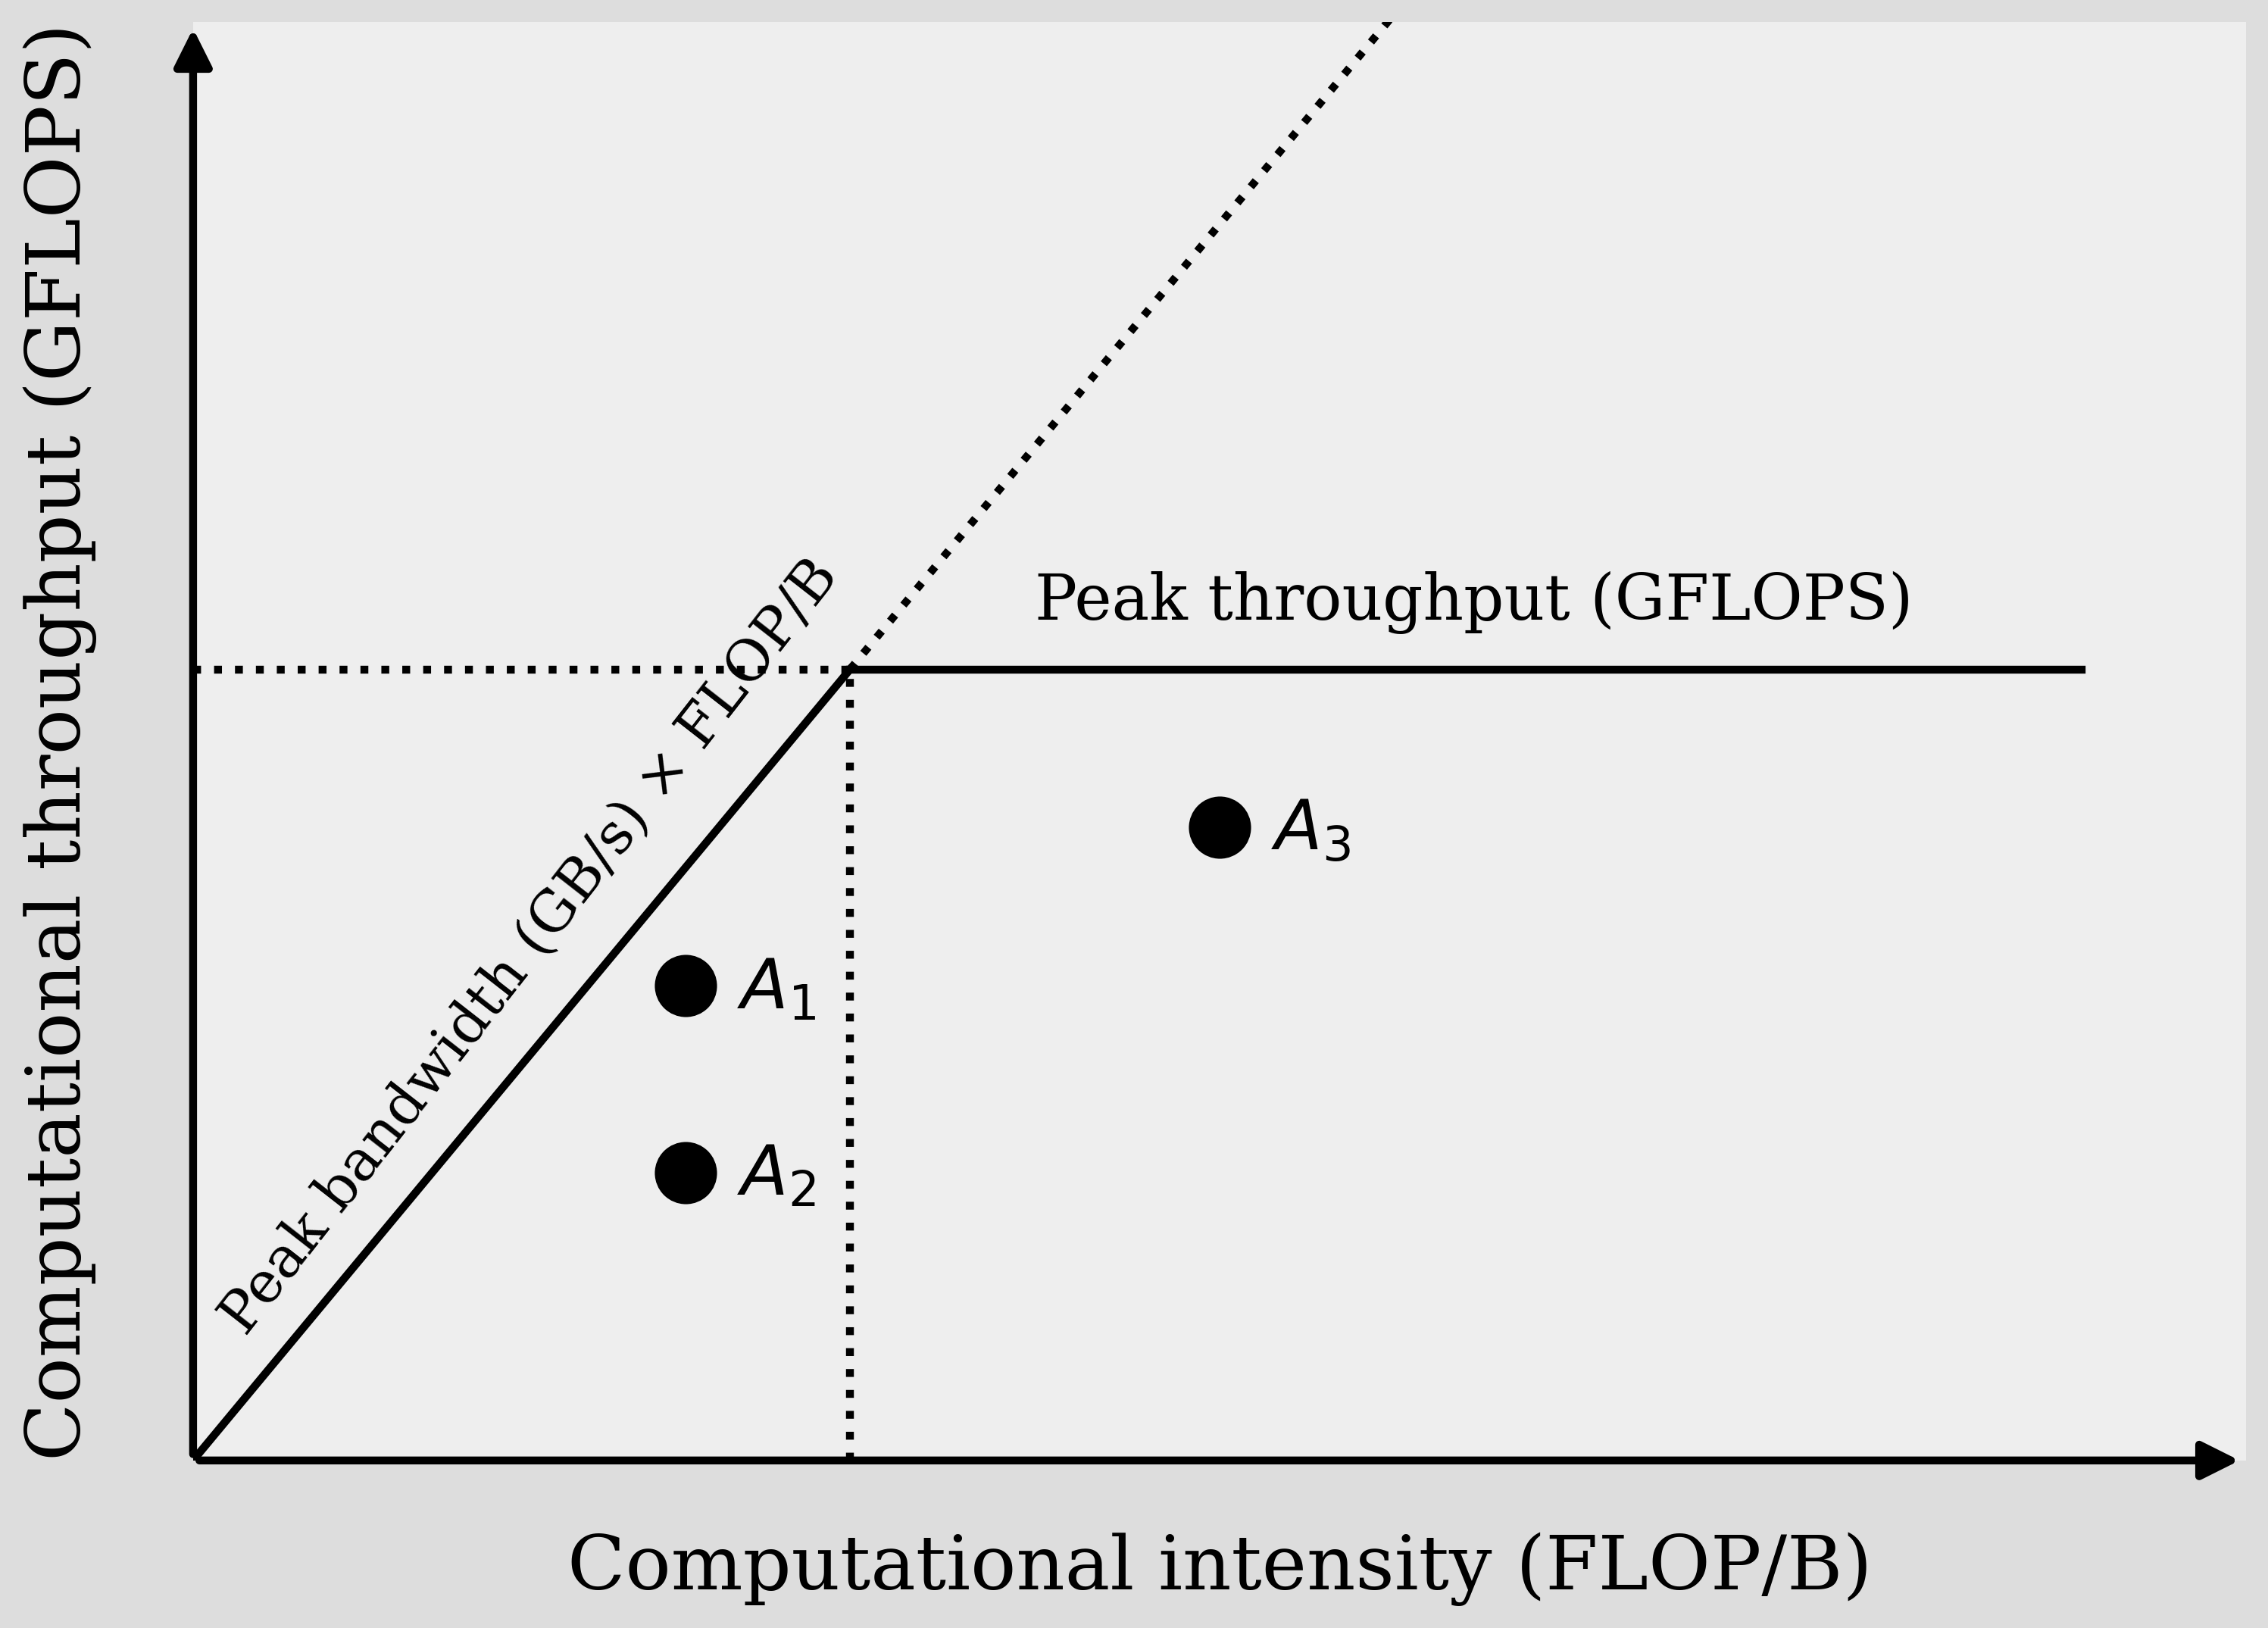
\includegraphics[width=0.58\textwidth]{fig1.png}
    \caption{Basic Roofline model. The sloped line is the memory-bandwidth limit and the horizontal line is the peak-compute limit.}
    \label{fig:roofline}
\end{figure}

The horizontal axis is \textbf{computational intensity}, measured in FLOP/B. Moving to the right means that every byte fetched from global memory supports more computation. The vertical axis is \textbf{achieved computational throughput}, usually measured in GFLOP/s or TFLOP/s.

The sloped line is the \textbf{memory-bandwidth roof}. Its equation is

\[
    P = B_{\text{peak}} I.
\]

At low computational intensity, throughput grows approximately in proportion to $I$: if each byte is reused more effectively, the same memory bandwidth can support more arithmetic work. This is the \textbf{memory-bound region}.

The horizontal line is the \textbf{compute roof},

\[
    P = P_{\text{peak}}.
\]

Once computational intensity is high enough, memory can theoretically feed the arithmetic units fast enough and the upper limit becomes the compute capability of the GPU. This is the \textbf{compute-bound region}. Together, the two limits give

\[
\boxed{
    P_{\text{achievable}}
    \leq
    \min\!\left(P_{\text{peak}},\,B_{\text{peak}}I\right)
}
\]

The intersection is the \textbf{ridge point}, where

\[
    I_{\text{ridge}}
    =
    \frac{P_{\text{peak}}}{B_{\text{peak}}}.
\]

The three points in Figure~\ref{fig:roofline} illustrate three different situations. \textbf{$A_1$ is memory bound but close to the sloped roof}, so the kernel is already using available memory bandwidth relatively efficiently; a major improvement requires higher data reuse and therefore higher computational intensity. \textbf{$A_2$ is also memory bound but lies far below the memory roof}; before changing the algorithm, its implementation should first improve memory-access efficiency, such as coalescing, occupancy, or memory-level parallelism. \textbf{$A_3$ lies in the high-intensity region and is mainly compute bound}; its next optimizations should focus on arithmetic utilization rather than simply reducing global-memory traffic.

\section{Data Reuse and the Preview of Tiling}

Matrix multiplication contains substantial inherent reuse. One element of $M$ participates in several output elements in the same output row, and one element of $N$ participates in several output elements in the same output column. A naive implementation allows different threads to request many of these values repeatedly from global memory.

The optimization target is therefore

\[
\begin{aligned}
&\text{load a value from global memory once} \\
&\qquad\downarrow \\
&\text{store it in fast on-chip memory} \\
&\qquad\downarrow \\
&\text{reuse it for many arithmetic operations}.
\end{aligned}
\]

Suppose a $T\times T$ thread block computes a $T\times T$ output tile. In one phase, the block loads one $T\times T$ tile from $M$ and one from $N$, so the global-memory traffic is

\[
    2T^2\times 4 = 8T^2\ \text{bytes}.
\]

The block has $T^2$ threads, and each thread performs $T$ multiply-add steps, giving

\[
    2T^3\ \text{FLOPs}.
\]

Thus the idealized intensity becomes

\[
\boxed{
    I_{\text{tiled}}
    =
    \frac{2T^3}{8T^2}
    =
    \frac{T}{4}\ \text{FLOP/B}
}
\]

instead of $0.25$ FLOP/B. The arithmetic workload is not reduced; the improvement comes from \textbf{reusing each value after it has been moved into on-chip shared memory}.

\section{A Short Performance Reasoning Procedure}

A practical Roofline-style analysis can be kept to four questions:

\begin{enumerate}
    \item How many useful FLOPs does the important loop or kernel perform?
    \item How many bytes must be read from or written to global memory?
    \item What is the computational intensity $I=\text{FLOPs}/\text{global-memory bytes}$?
    \item Is the measured kernel limited mainly by $B_{\text{peak}}I$ or by $P_{\text{peak}}$, and how far is it below that relevant roof?
\end{enumerate}

If a kernel is close to the bandwidth roof, the main route forward is usually more data reuse. If it is far below the bandwidth roof, memory accesses are not yet efficient. If it is close to the compute roof, arithmetic execution becomes the primary optimization target.

\section{CUDA Memory Types and Their Relationship to the Execution Hierarchy}

A CUDA device executes kernels as grids. A grid consists of many thread blocks, and every block contains many threads. \textbf{Registers are private to individual threads}, while \textbf{shared memory is allocated per block and can be accessed cooperatively by all threads in that block}. Global memory and constant memory are device-wide spaces: threads from different blocks can access them, and the host can transfer data to or from these device memory spaces using CUDA APIs.

This hierarchy is important because the memory location determines both performance and sharing behavior. The classical von Neumann picture already distinguishes a small register file close to the ALU from a much larger memory system farther away. CUDA makes this distinction especially important: \textbf{the register file and shared memory are on-chip resources inside the GPU, while global memory is normally implemented in off-chip DRAM such as GDDR or HBM}. Accessing a register operand can feed an arithmetic instruction directly; obtaining a global-memory operand requires address generation, a memory transaction, and a much longer trip through the memory hierarchy.

\subsection{Registers}

\textbf{Registers are the fastest storage normally visible to a CUDA thread.} They are on-chip and private to one thread. Loop counters, indices, pointer variables, and scalar accumulators such as \texttt{Pvalue} are commonly placed in registers. Their main limitation is capacity: the register file of an SM is finite, so high per-thread register usage can reduce the number of simultaneously resident blocks and warps. If the compiler cannot keep all thread-private values in registers, some values may be spilled into local memory.

\subsection{Local memory}

\textbf{Local memory is private in scope but not necessarily local in physical location.} The word ``local'' means that each thread has its own logical data, but local memory is normally backed by the device-memory hierarchy and is therefore much more expensive than registers. Large thread-private arrays, runtime-indexed arrays, stack data, or spilled registers may be placed there. It should not be confused with a small on-chip scratchpad.

\subsection{Shared memory}

\textbf{Shared memory is an explicitly managed on-chip memory allocated per block.} Every thread in the same block can read or write the same shared-memory array, while different blocks receive independent copies. This makes shared memory the key cooperation space for tiling: threads can cooperatively load a small working set from global memory, synchronize, reuse the data many times, and then overwrite the same shared-memory storage with the next working set. Because one thread may consume data written by another thread, shared-memory algorithms frequently require \texttt{\_\_syncthreads()} barriers.

\subsection{Global memory}

\textbf{Global memory is large, device-wide, and normally off-chip.} It stores the main input and output arrays of many CUDA programs and can be accessed by threads in any block. Its capacity is much larger than registers or shared memory, but its latency is much higher and its total throughput is limited by memory bandwidth. For performance-sensitive kernels, the key question is therefore not whether global memory can hold the data, but how often the same data must be fetched from it.

\subsection{Constant memory}

\textbf{Constant memory is a small device-wide read-only space for kernel code.} It is cached and is especially effective when threads in the same warp read the same constant address, because the value can be broadcast. It is useful for small coefficient tables or parameters that are initialized by the host and then reused by many threads without modification. The textbook capacity is $64$ KiB.

\subsection{One example containing the main memory spaces}

The following example is sufficient to show how the declarations map onto the CUDA memory hierarchy:

\begin{lstlisting}
__device__ float globalScale;
__constant__ float coefficients[256];

__global__ void memoryExample(
    const float* input,
    float* output,
    int n)
{
    __shared__ float tile[256];

    int tx = threadIdx.x;
    int tid = blockIdx.x * blockDim.x + tx;

    float value = 0.0f;

    if (tid < n) {
        tile[tx] = input[tid];
    }

    __syncthreads();

    if (tid < n) {
        value = tile[tx]
              * coefficients[tx]
              * globalScale;

        output[tid] = value;
    }
}
\end{lstlisting}

Here, \texttt{globalScale} resides in device global memory, \texttt{coefficients} resides in constant memory, and the arrays addressed by \texttt{input} and \texttt{output} are global-memory data. The array \texttt{tile} is one shared-memory object per block. The variables \texttt{tx}, \texttt{tid}, and \texttt{value} are private to each thread and are normally stored in registers. This one kernel therefore shows the most important distinction: \textbf{global memory stores large device-wide data, shared memory enables block-level cooperation, and registers hold thread-private working values close to the arithmetic units.}

\section{Tiled Matrix Multiplication: From Mathematics to GPU Execution to CUDA Code}

The previous sections established the performance motivation for tiling: global-memory traffic is expensive, matrix multiplication contains substantial data reuse, and shared memory provides an explicitly managed on-chip space in which a thread block can reuse data. The tiled matrix-multiplication kernel is therefore best understood as a continuous chain from the original matrix equation, to a block-level algorithm, to a GPU execution strategy, and finally to CUDA code.

\subsection{1. Ordinary Matrix Multiplication and the Source of Data Reuse}

Consider the ordinary matrix product

\[
    P = MN,
\]

where $M$, $N$, and $P$ are square matrices of width $W$. One output element is

\[
\boxed{
    P_{i,j}
    =
    \sum_{k=0}^{W-1}
    M_{i,k}N_{k,j}
}
\]

so $P_{i,j}$ is the dot product between row $i$ of $M$ and column $j$ of $N$. A straightforward CUDA implementation assigns one thread to one output element. Thread $(i,j)$ therefore repeatedly loads one element from row $i$ of $M$ and one element from column $j$ of $N$ while $k$ moves through the shared dimension.

The important observation is that neighboring output elements require overlapping input data. For example,

\[
\begin{aligned}
P_{0,0}
&=
M_{0,0}N_{0,0}
+M_{0,1}N_{1,0}
+M_{0,2}N_{2,0}
+M_{0,3}N_{3,0},
\\
P_{0,1}
&=
M_{0,0}N_{0,1}
+M_{0,1}N_{1,1}
+M_{0,2}N_{2,1}
+M_{0,3}N_{3,1}.
\end{aligned}
\]

Both outputs reuse the complete row $M_{0,:}$. Similarly, outputs in the same column reuse elements from the corresponding column of $N$. In a naive kernel, different threads may request the same matrix elements from global memory again and again. The mathematical number of multiply-add operations is unavoidable, but the repeated movement of the same input values is not.

This is exactly the optimization opportunity introduced earlier in this chapter:

\[
\begin{aligned}
&\text{load a value from global memory once} \\
&\qquad\downarrow \\
&\text{keep it in fast on-chip storage} \\
&\qquad\downarrow \\
&\text{reuse it for several arithmetic operations}.
\end{aligned}
\]

Tiling reorganizes matrix multiplication around this reuse pattern.

\subsection{2. Block Matrix Multiplication}

Before considering CUDA, it is useful to rewrite matrix multiplication purely as a block-matrix algorithm. Let the tile width be $T$, and partition the three matrices into $T\times T$ submatrices. For example, if $W=4$ and $T=2$,

\[
M=
\begin{bmatrix}
M^{(0,0)} & M^{(0,1)} \\
M^{(1,0)} & M^{(1,1)}
\end{bmatrix},
\qquad
N=
\begin{bmatrix}
N^{(0,0)} & N^{(0,1)} \\
N^{(1,0)} & N^{(1,1)}
\end{bmatrix},
\]

and

\[
P=
\begin{bmatrix}
P^{(0,0)} & P^{(0,1)} \\
P^{(1,0)} & P^{(1,1)}
\end{bmatrix}.
\]

Each symbol such as $M^{(0,1)}$ now represents a complete $2\times2$ matrix block rather than one scalar element. The multiplication rule itself does not change. The same row-by-column rule can be applied at the level of tiles:

\[
\boxed{
P^{(b_y,b_x)}
=
\sum_{ph}
M^{(b_y,ph)}N^{(ph,b_x)}
}
\]

Here $b_y$ and $b_x$ select one output tile, while $ph$ moves along the shared dimension. For the $4\times4$, $T=2$ example,

\[
\begin{aligned}
P^{(0,0)}
&=M^{(0,0)}N^{(0,0)}
 +M^{(0,1)}N^{(1,0)},
\\
P^{(0,1)}
&=M^{(0,0)}N^{(0,1)}
 +M^{(0,1)}N^{(1,1)},
\\
P^{(1,0)}
&=M^{(1,0)}N^{(0,0)}
 +M^{(1,1)}N^{(1,0)},
\\
P^{(1,1)}
&=M^{(1,0)}N^{(0,1)}
 +M^{(1,1)}N^{(1,1)}.
\end{aligned}
\]

This block formulation explains why tiled matrix multiplication naturally proceeds in \textbf{phases}. One output tile is not usually produced from one pair of input tiles. Instead, the algorithm repeatedly selects one tile from $M$ and one matching tile from $N$, multiplies them, and accumulates the result into the same output tile.

If $W$ is exactly divisible by $T$, the number of phases is

\[
    N_{\text{phase}} = \frac{W}{T}.
\]

For arbitrary dimensions, the general expression is

\[
    N_{\text{phase}}
    =
    \left\lceil \frac{W}{T}\right\rceil.
\]

At the level of one output element, the same transformation can be written as

\[
\boxed{
P_{row,col}
=
\sum_{ph}
\sum_{k=0}^{T-1}
M_{row,\,phT+k}
N_{phT+k,\,col}
}
\]

when $W$ is divisible by $T$. The original long dot product has therefore been split into several shorter dot products. The outer index $ph$ selects a tile pair, while the inner index $k$ traverses the shared dimension inside the current pair of tiles.

\subsection{3. A Complete $4\times4$ Example with $T=2$}

Now consider the upper-left output tile

\[
P^{(0,0)}
=
\begin{bmatrix}
P_{0,0} & P_{0,1} \\
P_{1,0} & P_{1,1}
\end{bmatrix}.
\]

Because $W=4$ and $T=2$, this tile requires two phases:

\[
\boxed{
P^{(0,0)}
=
\underbrace{M^{(0,0)}N^{(0,0)}}_{\text{phase 0}}
+
\underbrace{M^{(0,1)}N^{(1,0)}}_{\text{phase 1}}
}
\]

In phase 0, the required input tiles are

\[
M^{(0,0)}=
\begin{bmatrix}
M_{0,0} & M_{0,1} \\
M_{1,0} & M_{1,1}
\end{bmatrix},
\qquad
N^{(0,0)}=
\begin{bmatrix}
N_{0,0} & N_{0,1} \\
N_{1,0} & N_{1,1}
\end{bmatrix}.
\]

The four output elements receive the phase-0 contributions

\[
\begin{aligned}
P_{0,0}^{(\text{partial})}
&=M_{0,0}N_{0,0}+M_{0,1}N_{1,0},
\\
P_{0,1}^{(\text{partial})}
&=M_{0,0}N_{0,1}+M_{0,1}N_{1,1},
\\
P_{1,0}^{(\text{partial})}
&=M_{1,0}N_{0,0}+M_{1,1}N_{1,0},
\\
P_{1,1}^{(\text{partial})}
&=M_{1,0}N_{0,1}+M_{1,1}N_{1,1}.
\end{aligned}
\]

The reuse is now explicit. For example, $M_{0,0}$ contributes to both $P_{0,0}$ and $P_{0,1}$, while $N_{0,0}$ contributes to both $P_{0,0}$ and $P_{1,0}$. Instead of fetching these values independently for each output element, a tiled algorithm can fetch them once into a shared working set and let several output calculations reuse them.

Phase 1 uses the next pair of tiles,

\[
M^{(0,1)}=
\begin{bmatrix}
M_{0,2} & M_{0,3} \\
M_{1,2} & M_{1,3}
\end{bmatrix},
\qquad
N^{(1,0)}=
\begin{bmatrix}
N_{2,0} & N_{2,1} \\
N_{3,0} & N_{3,1}
\end{bmatrix}.
\]

The same four output elements then receive

\[
\begin{aligned}
P_{0,0}
&\mathrel{+}=M_{0,2}N_{2,0}+M_{0,3}N_{3,0},
\\
P_{0,1}
&\mathrel{+}=M_{0,2}N_{2,1}+M_{0,3}N_{3,1},
\\
P_{1,0}
&\mathrel{+}=M_{1,2}N_{2,0}+M_{1,3}N_{3,0},
\\
P_{1,1}
&\mathrel{+}=M_{1,2}N_{2,1}+M_{1,3}N_{3,1}.
\end{aligned}
\]

After phase 1, all four dot products are complete. The key point is that tiling has not changed the mathematics. It has only reorganized one long dot product into a sequence of shorter tile-sized dot products so that the data needed by several outputs can be handled together.

\subsection{4. Mapping Tiles onto CUDA Blocks and Threads}

The block-matrix structure maps naturally onto the CUDA execution hierarchy. \textbf{One thread block is assigned one $T\times T$ output tile, and one thread is assigned one output element inside that tile.} A $T\times T$ block therefore contains $T^2$ threads and produces $T^2$ output values.

For the $T=2$ example, one block contains four threads:

\[
\begin{array}{c|cc}
& tx=0 & tx=1 \\
\hline
 ty=0 & P_{0,0} & P_{0,1} \\
 ty=1 & P_{1,0} & P_{1,1}
\end{array}
\]

For a general block, the global output coordinates of thread $(ty,tx)$ are

\[
\boxed{
row = blockIdx.y\cdot T + ty
}
\]

and

\[
\boxed{
col = blockIdx.x\cdot T + tx.
}
\]

Thus \texttt{blockIdx.y} and \texttt{blockIdx.x} choose the output tile, while \texttt{threadIdx.y} and \texttt{threadIdx.x} choose one element inside that tile.

The complete matrices $M$ and $N$ remain in \textbf{global memory} because they are large. During one phase, however, the block needs only one $T\times T$ tile of $M$ and one $T\times T$ tile of $N$. Those two temporary working sets are placed in \textbf{shared memory}. Each thread also owns one private accumulator, typically named \texttt{Pvalue}, which is normally kept in a \textbf{register}.

The resulting memory mapping is therefore

\[
\begin{aligned}
&\text{complete input matrices} &&\rightarrow&& \text{global memory}, \\
&\text{current reusable input tiles} &&\rightarrow&& \text{shared memory}, \\
&\text{one thread's partial output} &&\rightarrow&& \text{register}.
\end{aligned}
\]

This is an important architectural point: the tile itself is not a special CUDA object. A tile is an algorithmic partition of a matrix. CUDA realizes that partition by assigning one output tile to a block and using the block's shared memory as the on-chip storage for the current pair of input tiles.

\subsection{5. One Phase on the GPU: Cooperative Loading, Reuse, and Synchronization}

One phase has a fixed execution pattern. Assume a $T\times T$ thread block. There are $T^2$ threads and each input tile also contains $T^2$ elements. The threads can therefore load the tiles cooperatively: thread $(ty,tx)$ loads one element from the current $M$ tile and one element from the current $N$ tile.

For phase $ph$, the shared-memory entries are

\[
\boxed{
Mds_{ty,tx}
=
M_{row,\,phT+tx}
}
\]

and

\[
\boxed{
Nds_{ty,tx}
=
N_{phT+ty,\,col}.
}
\]

The first expression means that the phase index moves the $M$ tile horizontally from left to right. The output row is fixed, $phT$ selects the beginning column of the current tile, and $tx$ selects one column inside that tile. The second expression means that the phase index moves the $N$ tile vertically from top to bottom. The output column is fixed, $phT$ selects the beginning row of the tile, and $ty$ selects one row inside it.

After the cooperative loads, the block must execute

\begin{lstlisting}
__syncthreads();
\end{lstlisting}

because a thread will generally consume shared-memory values written by other threads. For example, thread $(0,0)$ may need $Mds[0][1]$, which was loaded by thread $(0,1)$, and $Nds[1][0]$, which was loaded by thread $(1,0)$. The first barrier therefore guarantees that \textbf{all shared-memory writes for the current tiles are complete before any thread starts reading those tiles for arithmetic}.

Once the tile is complete, thread $(ty,tx)$ computes the phase contribution to its own output element:

\[
\boxed{
Pvalue
\mathrel{+}=
\sum_{k=0}^{T-1}
Mds_{ty,k}Nds_{k,tx}
}
\]

Here $ty$ remains fixed, so the thread reads one row of the shared $M$ tile. The value $tx$ remains fixed, so the thread reads one column of the shared $N$ tile. The inner index $k$ walks through the shared dimension exactly as in ordinary matrix multiplication. The difference is that these repeated arithmetic operations now consume values from fast on-chip shared memory instead of repeatedly fetching them from global memory.

The partial result \texttt{Pvalue} is private to the thread and persists across all phases. After one phase, the thread does not write a partial result back to global memory. It simply keeps accumulating into the same register value until the complete dot product has been evaluated.

A second barrier is required after the arithmetic:

\begin{lstlisting}
__syncthreads();
\end{lstlisting}

The shared arrays \texttt{Mds} and \texttt{Nds} are reused in the next phase. A fast thread must not overwrite them with the next tile pair while another thread is still reading the current tiles. The second barrier therefore guarantees that \textbf{all reads of the current tiles are complete before the shared-memory storage is overwritten}.

One phase can therefore be remembered as

\[
\begin{aligned}
&\text{load one }M\text{ tile and one }N\text{ tile from global memory} \\
&\qquad\downarrow \\
&\text{store them cooperatively in shared memory} \\
&\qquad\downarrow \\
&\texttt{\_\_syncthreads()} \\
&\qquad\downarrow \\
&\text{each thread performs }T\text{ multiply-add steps} \\
&\qquad\downarrow \\
&\texttt{\_\_syncthreads()} \\
&\qquad\downarrow \\
&\text{reuse the same shared arrays for the next phase}.
\end{aligned}
\]

This cooperative organization explains the reduction in global-memory traffic. A naive $T\times T$ block performs approximately

\[
    N_{\text{load,naive}} = 2WT^2
\]

input element loads. In the tiled version there are $W/T$ phases, and each phase loads only $2T^2$ elements, giving

\[
\begin{aligned}
N_{\text{load,tiled}}
&=
\frac{W}{T}(2T^2) \\
&=
2WT.
\end{aligned}
\]

The ideal reduction factor is therefore

\[
\boxed{
\frac{N_{\text{load,naive}}}
     {N_{\text{load,tiled}}}
=T
}
\]

while the number of floating-point multiply-add operations is unchanged. Tiling therefore improves performance by reducing data movement and increasing computational intensity, not by reducing the mathematical amount of work.

\subsection{6. From the Mapping to CUDA Code}

Once the mathematical and architectural mapping is clear, the CUDA kernel is a direct translation. The following textbook-style version assumes square matrices and assumes that \texttt{Width} is divisible by \texttt{TILE\_WIDTH}.

\begin{lstlisting}
#define TILE_WIDTH 16

__global__ void matrixMulTiledKernel(
    const float* M,
    const float* N,
    float* P,
    int Width)
{
    __shared__ float Mds[TILE_WIDTH][TILE_WIDTH];
    __shared__ float Nds[TILE_WIDTH][TILE_WIDTH];

    int tx = threadIdx.x;
    int ty = threadIdx.y;

    int row = blockIdx.y * TILE_WIDTH + ty;
    int col = blockIdx.x * TILE_WIDTH + tx;

    float Pvalue = 0.0f;

    for (int ph = 0;
         ph < Width / TILE_WIDTH;
         ++ph)
    {
        Mds[ty][tx] =
            M[row * Width
              + ph * TILE_WIDTH
              + tx];

        Nds[ty][tx] =
            N[(ph * TILE_WIDTH + ty)
              * Width
              + col];

        __syncthreads();

        for (int k = 0;
             k < TILE_WIDTH;
             ++k)
        {
            Pvalue +=
                Mds[ty][k]
                * Nds[k][tx];
        }

        __syncthreads();
    }

    P[row * Width + col] = Pvalue;
}
\end{lstlisting}

The first part of the kernel establishes the output mapping. The variables \texttt{tx} and \texttt{ty} are the thread coordinates inside the block, while

\[
row = blockIdx.y\cdot T + ty,
\qquad
col = blockIdx.x\cdot T + tx
\]

identify the output element computed by that thread. The accumulator \texttt{Pvalue} is initialized once and remains private to the thread across all phases.

The outer loop

\begin{lstlisting}
for (int ph = 0;
     ph < Width / TILE_WIDTH;
     ++ph)
\end{lstlisting}

implements the block-matrix sum

\[
P^{(b_y,b_x)}
=
\sum_{ph}
M^{(b_y,ph)}N^{(ph,b_x)}.
\]

Within one phase, the $M$ loading expression

\begin{lstlisting}
Mds[ty][tx] =
    M[row * Width
      + ph * TILE_WIDTH
      + tx];
\end{lstlisting}

is the row-major one-dimensional form of

\[
Mds_{ty,tx}
=
M_{row,\,phT+tx}.
\]

Likewise,

\begin{lstlisting}
Nds[ty][tx] =
    N[(ph * TILE_WIDTH + ty)
      * Width
      + col];
\end{lstlisting}

is the row-major form of

\[
Nds_{ty,tx}
=
N_{phT+ty,\,col}.
\]

These two statements are not arbitrary indexing tricks. They are the direct element-wise realization of loading the tile pair $M^{(b_y,ph)}$ and $N^{(ph,b_x)}$ required by the current block-matrix product.

After the first synchronization barrier, the inner loop

\begin{lstlisting}
for (int k = 0;
     k < TILE_WIDTH;
     ++k)
{
    Pvalue +=
        Mds[ty][k]
        * Nds[k][tx];
}
\end{lstlisting}

computes one tile-sized partial dot product. The relationship between the original dot-product index $q$ and the tiled indices is

\[
\boxed{
q = phT + k.
}
\]

Thus the original loop over $q=0,\ldots,W-1$ has been split into an outer phase loop and an inner tile loop. The mathematics is unchanged; only the organization of data movement and reuse has changed.

After every phase has finished, the thread owns the complete result

\[
Pvalue=P_{row,col},
\]

and performs one final global-memory store:

\begin{lstlisting}
P[row * Width + col] = Pvalue;
\end{lstlisting}

The complete architectural data path is therefore

\[
\begin{aligned}
&\text{complete }M,N\text{ in global memory} \\
&\qquad\downarrow \\
&\text{one current tile pair in block-shared on-chip memory} \\
&\qquad\downarrow \\
&\text{many shared-memory multiply-add operations} \\
&\qquad\downarrow \\
&\text{one private running sum in each thread's register} \\
&\qquad\downarrow \\
&\text{one final }P_{row,col}\text{ store to global memory}.
\end{aligned}
\]

The central lesson is therefore not merely that a tiled kernel uses \texttt{\_\_shared\_\_} arrays. \textbf{Tiling is an algorithmic reorganization that makes the CUDA memory hierarchy match the reuse structure already present in matrix multiplication.} Large matrices stay in global memory, a block stages the current reusable working set in shared memory, and each thread keeps its own accumulator in registers. This reduces repeated global-memory traffic and allows each fetched value to support more useful arithmetic.


\section{Boundary Checks for Arbitrary Matrix Sizes}

The basic tiled kernel assumes that the matrix dimensions are exact multiples of \texttt{TILE\_WIDTH}. For arbitrary sizes, threads near the matrix boundaries may attempt to load nonexistent input elements or write nonexistent output elements. Every global-memory access therefore needs its own boundary condition.

For a general matrix multiplication

\[
A_{M\times K}B_{K\times N}=C_{M\times N},
\]

define

\[
row=blockIdx.y\cdot T+ty,
\qquad
col=blockIdx.x\cdot T+tx,
\]

and, in phase $ph$,

\[
A_{\mathrm{col}}=phT+tx,
\qquad
B_{\mathrm{row}}=phT+ty.
\]

The cooperative loads should then be guarded as follows:

\begin{lstlisting}
if (row < M && A_col < K)
    Ads[ty][tx] = A[row * K + A_col];
else
    Ads[ty][tx] = 0.0f;

if (B_row < K && col < N)
    Bds[ty][tx] = B[B_row * N + col];
else
    Bds[ty][tx] = 0.0f;
\end{lstlisting}

Invalid input positions are filled with zero so that the same shared-memory dot-product loop can still be used for an incomplete tile. The final output store is also guarded:

\begin{lstlisting}
if (row < M && col < N)
    C[row * N + col] = Pvalue;
\end{lstlisting}

A thread that does not produce a valid output element should not simply return before the block synchronization points, because it may still be responsible for loading shared-memory data needed by other threads. Boundary checks must therefore be applied to the individual memory accesses rather than by removing such threads from the tiled execution.

For arbitrary $K$, the number of phases is

\[
\boxed{
N_{\mathrm{phase}}
=
\left\lceil \frac{K}{T}\right\rceil
}
\]

which can be implemented using integer arithmetic as

\begin{lstlisting}
int num_phases =
    (K + TILE_WIDTH - 1) / TILE_WIDTH;
\end{lstlisting}

\section{Shared-Memory Usage and Occupancy}

Shared memory is fast, but it is also a limited per-SM hardware resource. If every block requires a large amount of shared memory, fewer blocks can reside simultaneously on one SM, which may reduce occupancy and the GPU's ability to hide latency.

For the basic tiled matrix-multiplication kernel with tile width $T$, two shared-memory tiles are allocated:

\[
Mds[T][T],
\qquad
Nds[T][T].
\]

For single-precision data, the shared-memory requirement per block is

\[
\boxed{
S_{\mathrm{block}}
=
2T^2\times 4\ \text{bytes}.
}
\]

For $T=16$,

\[
S_{\mathrm{block}}
=
2\times16^2\times4
=
2048\ \text{bytes}.
\]

This is relatively small, so the simple $16\times16$ tiled kernel is usually not limited by shared memory alone. In general, however, occupancy can be constrained jointly by shared memory, registers, the maximum number of resident warps, the maximum number of threads, and the maximum number of blocks per SM. Higher occupancy is therefore not automatically equivalent to higher performance; the important goal is to maintain enough active warps to hide latency while preserving efficient data reuse.

The declarations used so far allocate shared memory statically:

\begin{lstlisting}
__shared__ float Mds[TILE_WIDTH][TILE_WIDTH];
__shared__ float Nds[TILE_WIDTH][TILE_WIDTH];
\end{lstlisting}

Their sizes are fixed at compile time. CUDA also supports \textbf{dynamic shared memory}, whose size is selected when the kernel is launched:

\begin{lstlisting}
extern __shared__ float shared[];

float* Mds = shared;
float* Nds = shared
           + TILE_WIDTH * TILE_WIDTH;
\end{lstlisting}

The host supplies the required number of bytes as the third kernel-launch configuration argument:

\begin{lstlisting}
size_t shared_bytes =
    2 * TILE_WIDTH * TILE_WIDTH
      * sizeof(float);

kernel<<<grid, block, shared_bytes>>>(...);
\end{lstlisting}

Dynamic shared memory is useful when the amount of per-block scratch space should be chosen at runtime according to the kernel configuration or the resources available on a particular GPU. The broader principle is that \textbf{shared memory improves locality and reuse, but its capacity must be balanced against the number of blocks and warps that can remain resident on each SM}.

\end{document}
